\subsection{Hypothesis Generation} \label{sec:hypothesis-gen}

Coming up with new hypotheses represents a cornerstone of the scientific process \autocite{rock2018hypothesis}. Historically, hypotheses have emerged from systematic observation of natural phenomena, exemplified by Isaac Newton’s formulation of the law of universal gravitation \autocite{newton1999principia}, which was inspired by the seemingly mundane observation of a falling apple \autocite{kosso2017whatgoesup}.

In modern research, hypothesis generation increasingly relies on data-driven tools. 
For example, clinical research employs frameworks such as \gls{viads} to derive testable hypotheses from well-curated datasets \autocite{Jing2022roles}. Similarly, advances in \glspl{llm} are now being explored for their potential to automate and enhance idea generation across scientific domains \autocite{oneill2025sparks}. However, such approaches face significant challenges due to the inherently open-ended nature of scientific discovery \autocite{stanley2017openendedness}. 
Open-ended domains, as discussed in \Cref{sec:data-section}, risk intractability, as an unbounded combinatorial space of potential variables, interactions, and experimental parameters complicates systematic exploration \autocite{clune2019ai0gas0}.
Moreover, the quantitative evaluation of the novelty and impact of generated hypotheses remains non-trivial. 
As Karl Popper argued, scientific discovery defies rigid logical frameworks \autocite{popper1959logic}, and objective metrics for \enquote{greatness} of ideas are elusive \autocite{stanley2015greatness}. These challenges underscore the complexity of automating or systematizing the creative core of scientific inquiry.

\subsubsection{Initial Sparks}

Recent efforts in the \gls{ml} community have sought to simulate the hypothesis formulation process \autocite{Gu2025forecasting, arlt2024meta0designing}, primarily leveraging multi-agent systems \autocite{jansen2025codescientist0, kumbhar2025hypothesis}. 
In such frameworks, agents typically retrieve prior knowledge to contextualize previous related work---grounding hypothesis generation in existing literature \autocite{naumov2025dora, ghareeb2025robin0, gu2024interesting}. 
A key challenge, however, lies in evaluating the generated hypotheses. 
While some studies leverage \glspl{llm} to evaluate novelty or interestingness \autocite{zhang2024omni0}, recent work has introduced critic agents---specialized components designed to monitor and iteratively correct outputs from other agents---into multi-agent frameworks (see \Cref{sec:multi-agent}). 
For instance, \textcite{Ghafarollahi2024} demonstrated how integrating such critics enables systematic hypothesis refinement through continuous feedback mechanisms.

However, the reliability of purely model-based evaluation remains contentious. 
\textcite{si2025llms} argued that relying on a \gls{gpm} to evaluate hypotheses lacks robustness, advocating instead for human assessment. 
This approach was adopted in their work, where human evaluators validated hypotheses produced by their system, finding more novel \gls{llm}-produced hypotheses compared to the ones proposed by humans.
Notably, \textcite{yamada2025ai} advanced the scope of such systems by automating the entire research \gls{ml} process, from hypothesis generation to article writing. 
Their system’s outputs were submitted to workshops at the \gls{iclr} 2025, with one contribution ultimately accepted. However, the advancements made by such works are currently incremental instead of unveiling new, paradigm-shifting  research (see \Cref{fig:hypothesis-generation}).

\subsubsection{Chemistry-Focused Hypotheses}

In scientific fields such as chemistry and materials science, hypothesis generation requires domain intuition, mastery of specialized terminology, and the ability to reason through foundational concepts \autocite{miret2024llms}. 
To address potential knowledge gaps in \glspl{llm}, \textcite{wang2023scimon0} proposed a few-shot learning approach (see \Cref{sec:prompting}) for hypothesis generation and compared it with model fine-tuning for the same task. 
Their method strategically incorporates in-context examples to supplement domain knowledge while discouraging over-reliance on existing literature. 
For fine-tuning, they designed a loss function that penalizes possible biases---e.g., given the context \enquote{hierarchical tables challenge numerical reasoning}, the model would be penalized if it generated an overly generic prediction like \enquote{table analysis} instead of a task-specific one---when trained on such examples. 
Human evaluations of ablation studies revealed that \modelname{GPT-4}, augmented with a knowledge graph of prior research, outperformed fine-tuned models in generating hypotheses with greater technical specificity and iterative refinement of such hypotheses.

Complementing this work, \textcite{yang2025moose} introduced the \modelname{Moose-Chem} framework to evaluate the novelty of \gls{llm}-generated hypotheses. 
To avoid data contamination, their benchmark exclusively uses papers published after the knowledge cutoff date of the evaluated model, \modelname{GPT-4o}. 
Ground-truth hypotheses were derived from articles in high-impact journals (e.g., Nature, Science) and validated by domain-specialized PhD researchers.
By iteratively providing the model with context from prior studies, \modelname{GPT-4o} achieved coverage of over $80\%$ of the evaluation set’s hypotheses while accessing only $4\%$ of the retrieval corpus, demonstrating efficient synthesis of ideas presumably not present in its training corpus.

\begin{figure}[!ht]
    \centering
        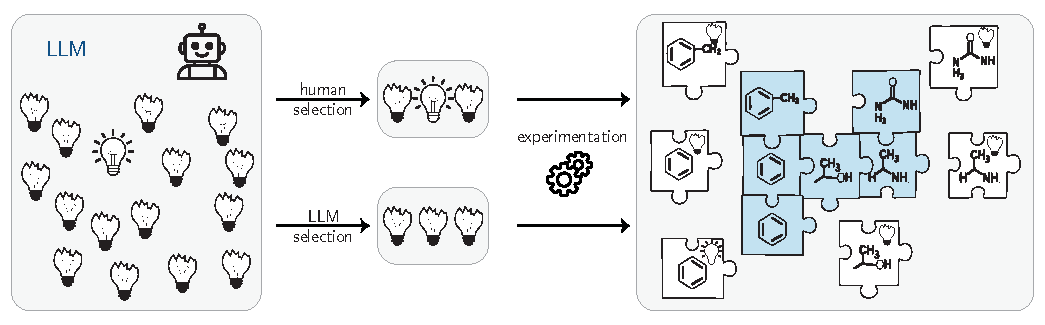
\includegraphics[width=1\textwidth]{figures/rescaled_figures/chemrev_figure13.pdf}
    \caption{\textbf{Overview of \gls{llm}-based hypothesis generation}. 
    Current methods are based on \gls{llm}-sampling methods in which an \gls{llm} proposes new hypotheses. 
    The generated hypotheses are evaluated in terms of novelty and impact either by another \gls{llm} or by a human. Then, through experimentation, the hypotheses are transformed into results which showcase that current \glspl{llm} cannot produce groundbreaking ideas, limited to their training corpus, resulting in the best cases, in incremental work. This is shown metaphorically with the puzzle. The \enquote{pieces of chemical knowledge} based on the hypothesis produced by \glspl{llm} are already present in the \enquote{chemistry puzzle}, not unveiling new parts of it.}
    \label{fig:hypothesis-generation}
\end{figure}

\subsubsection{Are LLMs Actually Capable of Novel Hypothesis Generation?}

Automatic hypothesis generation is often regarded as the Holy Grail of automating the scientific process \autocite{coley2020autonomous}. However, achieving this milestone remains challenging, as generating novel and impactful ideas requires questioning current scientific paradigms \autocite{Kuhn1962Structure}---a skill typically refined through years of experience---which is currently impossible for most \gls{ml} systems.

Current progress in \gls{ml} illustrates these limitations \autocite{kon2025exp0bench0, gu2024interesting}. Although some studies claim success in \gls{ai}-generated ideas accepted at workshops in \gls{ml} conferences via double-blind review \autocite{zhou2025tempest0}, these achievements are limited. 
First, accepted submissions often focus on coding tasks, one of the strongest domains for \glspl{llm}. Second, workshop acceptances are less competitive than main conferences, as they prioritize early-stage ideas over rigorously validated contributions. 
In chemistry, despite some works showing promise on these systems \autocite{yang2025moose0chem20}, \glspl{llm} struggle to propose functional hypotheses \autocite{si2025ideation1execution}.
Their apparent success often hinges on extensive sampling and iterative refinement, rather than genuine conceptual innovation.

As \textcite{Kuhn1962Structure} argued, generating groundbreaking ideas demands challenging prevailing paradigms---a capability missing in current \gls{ml} models (they are trained to make the existing paradigm more likely in training rather than questioning their training data), as shown in \Cref{fig:hypothesis-generation}. 
Thus, while accidental discoveries can arise from non-programmed events (e.g., Fleming’s identification of penicillin \autocite{Fleming1929antibacterial, Fleming1945penicillin}), transformative scientific advances typically originate from deliberate critique of existing knowledge \autocite{popper1959logic, Lakatos1970falsification}. In addition, very often breakthroughs can also not be achieved by optimizing for a simple metric---as we often do not fully understand the problem and, hence, cannot design a metric.\autocite{stanley2015greatness}
Despite some publications suggesting that \gls{ai} scientists already exist, such claims are supported only by narrow evaluations that yield incremental progress \autocite{novikov2025alphaevolve}, not paradigm-shifting insights. For \gls{ai} to evolve from research assistants into autonomous scientists, it must demonstrate efficacy in addressing societally consequential challenges, such as solving complex, open-ended problems at scale (e.g., \enquote{millennium} math problems
\autocite{Carlson2006millennium}).

Finally, ethical considerations become critical as hypothesis generation grows more data-driven and automated. Adherence to legal and ethical standards must guide these efforts (see \Cref{sec:safety}) \autocite{danish_gov2024hypothesis}.

With a hypothesis in hand, the next step is often to run an experiment to test it. 